\documentclass[10pt,letterpaper]{article}
%DIF LATEXDIFF DIFFERENCE FILE


\usepackage[top=0.85in,left=2.75in,footskip=0.75in]{geometry}
%DIF 3-4c3-5
%DIF < \usepackage{setspace}
%DIF < \doublespacing
%DIF -------
 %DIF > 
%\usepackage{setspace} %DIF > 
%\doublespacing %DIF > 
%DIF -------
% amsmath and amssymb packages, useful for mathematical formulas and symbols
\usepackage{amsmath,amssymb}
\usepackage{enumitem}
% Use adjustwidth environment to exceed column width (see example table in text)
\usepackage{changepage}

% Use Unicode characters when possible
\usepackage[utf8x]{inputenc}

% textcomp package and marvosym package for additional characters
\usepackage{textcomp,marvosym}

% cite package, to clean up citations in the main text. Do not remove.
\usepackage{cite}

% Use nameref to cite supporting information files (see Supporting Information section for more info)
\usepackage{nameref,hyperref}
\usepackage[table]{xcolor}
% line numbers
\usepackage[right]{lineno}

% ligatures disabled
\usepackage{microtype}
\DisableLigatures[f]{encoding = *, family = * }

% color can be used to apply background shading to table cells only
\usepackage[table]{xcolor}

% array package and thick rules for tables
\usepackage{array}
\usepackage{multirow}
\usepackage{booktabs}
\usepackage{tabularx}
\usepackage{array} % for defining a new column type
\usepackage{varwidth} %for the varwidth minipage environment
\usepackage{makecell}
\usepackage{booktabs, cellspace, hhline}
\setlength\cellspacetoplimit{24pt}
\setlength\cellspacebottomlimit{4pt}

\newcolumntype{+}{!{\vrule width 2pt}}


\newlength\savedwidth
\newcommand\thickcline[1]{%
  \noalign{\global\savedwidth\arrayrulewidth\global\arrayrulewidth 2pt}%
  \cline{#1}%
  \noalign{\vskip\arrayrulewidth}%
  \noalign{\global\arrayrulewidth\savedwidth}%
}

\newcommand\thickhline{\noalign{\global\savedwidth\arrayrulewidth\global\arrayrulewidth 2pt}%
\hline
\noalign{\global\arrayrulewidth\savedwidth}}



\raggedright
\setlength{\parindent}{0.5cm}
\textwidth 5.25in 
\textheight 8.75in

\usepackage[aboveskip=1pt,labelfont=bf,labelsep=period,justification=raggedright,singlelinecheck=off]{caption}
\renewcommand{\figurename}{Fig}

\bibliographystyle{plos2015}

\makeatletter
\renewcommand{\@biblabel}[1]{\quad#1.}
\makeatother

\usepackage{lastpage,fancyhdr,graphicx}
\usepackage{epstopdf}
%\pagestyle{myheadings}
\pagestyle{fancy}
\fancyhf{}
%\setlength{\headheight}{27.023pt}
%\lhead{%\includegraphics[width=2.0in]{PLOS-submission.eps}}
\rfoot{\thepage/\pageref{LastPage}}
\renewcommand{\headrulewidth}{0pt}
\renewcommand{\footrule}{\hrule height 2pt \vspace{2mm}}
\fancyheadoffset[L]{2.25in}
\fancyfootoffset[L]{2.25in}
\lfoot{\today}

%DIF 90-91d91
%DIF < \newcommand{\lorem}{{\bf LOREM}}
%DIF < \newcommand{\ipsum}{{\bf IPSUM}}
%DIF -------


%DIF < \newcommand{\blue\numbera}{58.5\% }
%DIF -------
\input{../R_results/paper_estimates1.tex} %DIF > 
%DIF < \newcommand{\blue\numberb}{14.8\% }
\input{../R_results/paper_estimates2.tex} %DIF > 
%DIF < \newcommand{\blue\numberc}{35.1\% }
\input{../R_results/paper_estimates3.tex} %DIF > 
%DIF < 
\input{../R_results/paper_estimates4.tex} %DIF > 
%DIF < \newcommand{\blue\numberda}{46.8\% }
%DIF < \newcommand{\blue\numberdb}{19.7\%-54.5\%}
%DIF < \newcommand{\blue\numberea}{58.5\% }
%DIF < \newcommand{\blue\numbereb}{32.5\%-68.9\%}
%DIF < \newcommand{\blue\numberfa}{14.3\% }
%DIF < \newcommand{\blue\numberfb}{3.5\%-17.5\%}
%DIF < \newcommand{\blue\numberga}{14.8\% }
%DIF < \newcommand{\blue\numbergb}{6.6\%-19.5\%}
%DIF < 
%DIF < \newcommand{\blue\numberha}{23.9\% }
%DIF < \newcommand{\blue\numberhb}{7.7\%-29.3\%}
%DIF < \newcommand{\blue\numberia}{35.1\% }
%DIF < \newcommand{\blue\numberib}{17.0\%-48.7\%}
%DIF < 
%DIF < \newcommand{\blue\numberja}{14.5\% }
%DIF < \newcommand{\blue\numberjb}{48.8\%}
%DIF < 
%DIF < \newcommand{\blue\numberk}{42.4\% }
%DIF < \newcommand{\blue\numberl}{32.3\% }
%DIF < \newcommand{\blue\numberm}{28.7\% }
%DIF < \newcommand{\blue\numbern}{25.5\% }
%DIF < 
%DIF < \newcommand{\blue\numbero}{23.9\% }
%DIF < \newcommand{\blue\numberp}{34.8\% }
%DIF PREAMBLE EXTENSION ADDED BY LATEXDIFF
%DIF UNDERLINE PREAMBLE %DIF PREAMBLE
\RequirePackage[normalem]{ulem} %DIF PREAMBLE
\RequirePackage{color}\definecolor{RED}{rgb}{1,0,0}\definecolor{BLUE}{rgb}{0,0,1} %DIF PREAMBLE
\providecommand{\DIFaddtex}[1]{{\protect\color{blue}\uwave{#1}}} %DIF PREAMBLE
\providecommand{\DIFdeltex}[1]{{\protect\color{red}\sout{#1}}}                      %DIF PREAMBLE
%DIF SAFE PREAMBLE %DIF PREAMBLE
\providecommand{\DIFaddbegin}{} %DIF PREAMBLE
\providecommand{\DIFaddend}{} %DIF PREAMBLE
\providecommand{\DIFdelbegin}{} %DIF PREAMBLE
\providecommand{\DIFdelend}{} %DIF PREAMBLE
%DIF FLOATSAFE PREAMBLE %DIF PREAMBLE
\providecommand{\DIFaddFL}[1]{\DIFadd{#1}} %DIF PREAMBLE
\providecommand{\DIFdelFL}[1]{\DIFdel{#1}} %DIF PREAMBLE
\providecommand{\DIFaddbeginFL}{} %DIF PREAMBLE
\providecommand{\DIFaddendFL}{} %DIF PREAMBLE
\providecommand{\DIFdelbeginFL}{} %DIF PREAMBLE
\providecommand{\DIFdelendFL}{} %DIF PREAMBLE
%DIF HYPERREF PREAMBLE %DIF PREAMBLE
\providecommand{\DIFadd}[1]{\texorpdfstring{\DIFaddtex{#1}}{#1}} %DIF PREAMBLE
\providecommand{\DIFdel}[1]{\texorpdfstring{\DIFdeltex{#1}}{}} %DIF PREAMBLE
\newcommand{\DIFscaledelfig}{0.5}
%DIF HIGHLIGHTGRAPHICS PREAMBLE %DIF PREAMBLE
\RequirePackage{settobox} %DIF PREAMBLE
\RequirePackage{letltxmacro} %DIF PREAMBLE
\newsavebox{\DIFdelgraphicsbox} %DIF PREAMBLE
\newlength{\DIFdelgraphicswidth} %DIF PREAMBLE
\newlength{\DIFdelgraphicsheight} %DIF PREAMBLE
% store original definition of \includegraphics %DIF PREAMBLE
\LetLtxMacro{\DIFOincludegraphics}{\includegraphics} %DIF PREAMBLE
\newcommand{\DIFaddincludegraphics}[2][]{{\color{blue}\fbox{\DIFOincludegraphics[#1]{#2}}}} %DIF PREAMBLE
\newcommand{\DIFdelincludegraphics}[2][]{% %DIF PREAMBLE
\sbox{\DIFdelgraphicsbox}{\DIFOincludegraphics[#1]{#2}}% %DIF PREAMBLE
\settoboxwidth{\DIFdelgraphicswidth}{\DIFdelgraphicsbox} %DIF PREAMBLE
\settoboxtotalheight{\DIFdelgraphicsheight}{\DIFdelgraphicsbox} %DIF PREAMBLE
\scalebox{\DIFscaledelfig}{% %DIF PREAMBLE
\parbox[b]{\DIFdelgraphicswidth}{\usebox{\DIFdelgraphicsbox}\\[-\baselineskip] \rule{\DIFdelgraphicswidth}{0em}}\llap{\resizebox{\DIFdelgraphicswidth}{\DIFdelgraphicsheight}{% %DIF PREAMBLE
\setlength{\unitlength}{\DIFdelgraphicswidth}% %DIF PREAMBLE
\begin{picture}(1,1)% %DIF PREAMBLE
\thicklines\linethickness{2pt} %DIF PREAMBLE
{\color[rgb]{1,0,0}\put(0,0){\framebox(1,1){}}}% %DIF PREAMBLE
{\color[rgb]{1,0,0}\put(0,0){\line( 1,1){1}}}% %DIF PREAMBLE
{\color[rgb]{1,0,0}\put(0,1){\line(1,-1){1}}}% %DIF PREAMBLE
\end{picture}% %DIF PREAMBLE
}\hspace*{3pt}}} %DIF PREAMBLE
} %DIF PREAMBLE
\LetLtxMacro{\DIFOaddbegin}{\DIFaddbegin} %DIF PREAMBLE
\LetLtxMacro{\DIFOaddend}{\DIFaddend} %DIF PREAMBLE
\LetLtxMacro{\DIFOdelbegin}{\DIFdelbegin} %DIF PREAMBLE
\LetLtxMacro{\DIFOdelend}{\DIFdelend} %DIF PREAMBLE
\DeclareRobustCommand{\DIFaddbegin}{\DIFOaddbegin \let\includegraphics\DIFaddincludegraphics} %DIF PREAMBLE
\DeclareRobustCommand{\DIFaddend}{\DIFOaddend \let\includegraphics\DIFOincludegraphics} %DIF PREAMBLE
\DeclareRobustCommand{\DIFdelbegin}{\DIFOdelbegin \let\includegraphics\DIFdelincludegraphics} %DIF PREAMBLE
\DeclareRobustCommand{\DIFdelend}{\DIFOaddend \let\includegraphics\DIFOincludegraphics} %DIF PREAMBLE
\LetLtxMacro{\DIFOaddbeginFL}{\DIFaddbeginFL} %DIF PREAMBLE
\LetLtxMacro{\DIFOaddendFL}{\DIFaddendFL} %DIF PREAMBLE
\LetLtxMacro{\DIFOdelbeginFL}{\DIFdelbeginFL} %DIF PREAMBLE
\LetLtxMacro{\DIFOdelendFL}{\DIFdelendFL} %DIF PREAMBLE
\DeclareRobustCommand{\DIFaddbeginFL}{\DIFOaddbeginFL \let\includegraphics\DIFaddincludegraphics} %DIF PREAMBLE
\DeclareRobustCommand{\DIFaddendFL}{\DIFOaddendFL \let\includegraphics\DIFOincludegraphics} %DIF PREAMBLE
\DeclareRobustCommand{\DIFdelbeginFL}{\DIFOdelbeginFL \let\includegraphics\DIFdelincludegraphics} %DIF PREAMBLE
\DeclareRobustCommand{\DIFdelendFL}{\DIFOaddendFL \let\includegraphics\DIFOincludegraphics} %DIF PREAMBLE
%DIF END PREAMBLE EXTENSION ADDED BY LATEXDIFF
\newcommand{\blue}[1]{\textcolor{blue}{#1}}
\begin{document}








\vspace*{0.2in}

\begin{flushleft}
{\Large
\textbf\newline{The Impact of Scaling up Dolutegravir on Antiretroviral Resistance in South Africa} 
}
\newline
\\
Anthony Hauser\textsuperscript{1},
Katharina Kusejko\textsuperscript{2},
Leigh F. Johnson\textsuperscript{3},
Huldrych F. Günthard\textsuperscript{2,4},
Julien Riou\textsuperscript{1},
Gilles Wandeler\textsuperscript{1,5},
Matthias Egger\textsuperscript{1,3,*},
Roger D. Kouyos\textsuperscript{2,4,*}
\\
\bigskip
\textbf{1} Institute of Social and Preventive Medicine, University of Bern, Switzerland
\\
\textbf{2} Division of Infectious Diseases and Hospital Epidemiology, University Hospital Zurich, University of Zurich, Zurich, Switzerland
\\
\textbf{3} Centre for Infectious Disease Epidemiology and Research, University of Cape Town, South Africa
\\
\textbf{4} Institute of Medical Virology, University of Zurich, Zurich, Switzerland
\\
\textbf{5} Department of Infectious Diseases, Bern University Hospital, University of Bern, Bern, Switzerland
\\
\bigskip
* matthias.egger@ispm.unibe.ch or roger.kouyos@uzh.ch

\end{flushleft}
\DIFaddbegin 


\DIFaddend \section*{Abstract}
\subsection*{Background} Rising resistance of HIV-1 to non-nucleoside reverse transcriptase inhibitors (NNRTIs) threatens the success of the global scale-up of antiretroviral therapy (ART). The switch to WHO-recommended dolutegravir (DTG)-based regimens could reduce this threat due to DTG’s high genetic barrier to resistance. We used mathematical modelling to \DIFdelbegin \DIFdel{examine }\DIFdelend \DIFaddbegin \DIFadd{predict }\DIFaddend the impact of the scale-up of DTG-based ART on NNRTI pre-treatment drug resistance (PDR) in South Africa, \DIFdelbegin \DIFdel{2019-2040}\DIFdelend \DIFaddbegin \DIFadd{2020-2040}\DIFaddend .

\subsection*{Methods and \DIFdelbegin \DIFdel{results}\DIFdelend \DIFaddbegin \DIFadd{Findings}\DIFaddend }
We adapted the MARISA (Modelling Antiretroviral drug Resistance In South Africa) model, an epidemiological model of the transmission of NNRTI resistance in South Africa. We modelled the introduction of DTG in \DIFdelbegin \DIFdel{2019 }\DIFdelend \DIFaddbegin \DIFadd{2020 }\DIFaddend under two scenarios: DTG as first-line regimen for ART-initiators, or DTG for all patients, including patients on suppressive NNRTI-based ART. Due to safety concerns related to DTG during pregnancy, we assessed the impact of prescribing DTG to all men and in addition to i) women beyond reproductive age, ii) women beyond reproductive age or using contraception, and iii) all women. The model projections show that, compared to the continuation of NNRTI-based ART, introducing DTG would lead to a reduction in NNRTI \DIFdelbegin \DIFdel{resistance }\DIFdelend \DIFaddbegin \DIFadd{pre-treatment drug resistance (PDR) }\DIFaddend in all scenarios if both ART initiators are started on a DTG-based regimens and those on NNRTI-based regimens are rapidly switched to DTG. NNRTI \DIFdelbegin \DIFdel{resistance }\DIFdelend \DIFaddbegin \DIFadd{PDR }\DIFaddend would continue to increase if DTG-based ART was restricted to men. When given to all men and women, DTG-based ART could reduce the level of NNRTI \DIFdelbegin \DIFdel{resistance }\DIFdelend \DIFaddbegin \DIFadd{PDR }\DIFaddend from \blue\numbera (without DTG) to \blue\numberb (with universal DTG) in 2040. If \DIFdelbegin \DIFdel{all }\DIFdelend \DIFaddbegin \DIFadd{only }\DIFaddend men and women beyond reproductive age or on contraception are started on or switched to DTG-based ART, NNRTI \DIFdelbegin \DIFdel{resistance }\DIFdelend \DIFaddbegin \DIFadd{PDR }\DIFaddend would reach \blue\numberc in 2040. \DIFaddbegin \DIFadd{Limitations include high uncertainty due to the long-term predictions and the current scarcity of knowledge about DTG efficacy in South Africa.
}\DIFaddend \subsection*{Conclusions}
Our model shows the potential benefit of scaling up DTG-based regimens for halting the rise of NNRTI resistance. Starting or switching all men and women to DTG would lead to a sustained decline in resistance levels whereas using DTG-based ART in all men, or in men and women beyond childbearing age, would \DIFaddbegin \DIFadd{only }\DIFaddend slow down the increase in levels of NNRTI \DIFdelbegin \DIFdel{resistance.
}\DIFdelend \DIFaddbegin \DIFadd{PDR.
}\section*{\DIFadd{Author summary}}
\textbf{\DIFadd{Why was this study done?}}
\begin{itemize}
\item \DIFadd{The scale-up of antiretroviral therapy in resource-limited settings has achieved an unprecedented reduction in HIV-related morbidity and mortality. 
}\item \DIFadd{The success of antiretroviral therapy is however threatened by increasing levels of resistance to antiretroviral drugs of the non-nucleoside reverse transcriptase inhibitors (NNRTI) class. 
}\item \DIFadd{Replacing NNRTIs by dolutegravir may curb the spread of resistance but it is unclear how effective this switch will be and which patient groups should be switched from NNRTI to dolutegravir. 
}\item \DIFadd{It has been debated whether Dolutegravir should be given to women, because of a potential risk of birth defects, and to patients already on an NNRTI based therapy.
}\end{itemize}
\textbf{\DIFadd{What did the researchers do and find?}}
\begin{itemize}
\item \DIFadd{Using a mathematical model simulating the HIV epidemic in South Africa, we find that scaling up dolutegravir-based antiretroviral therapy can halt the increase of NNRTI resistance.
}\item \DIFadd{This beneficial effect of dolutegravir depends crucially on including both women and people already on NNRTI-based ART among patients to whom dolutegravir will be prescribed. 
}\item \DIFadd{Restricting dolutegravir to men or to patients initiating antiretroviral therapy would substantially reduce its potential to curb resistance at the population level, as in this case it could merely slow down but not halt the spread of NNRTI resistance. 
}\item \DIFadd{Patients still relying on NNRTI-based therapy would in this case face increased risk of resistance and therapy failure.
}\end{itemize}
\textbf{\DIFadd{What do these findings mean?}}
\begin{itemize}
\item \DIFadd{Our model highlights the potential of dolutegravir scale up to curb NNRTI resistance. 
}\item \DIFadd{In order to halt the increase in NNRTI resistance, dolutegravir should become accessible to both women and people currently on NNRTI-based therapy.
}\end{itemize}
\DIFaddend 


\linenumbers
\DIFdelbegin %DIFDELCMD < 

%DIFDELCMD < %%%
\DIFdelend \section*{Introduction}
The rollout of antiretroviral therapy in South Africa is estimated to have prevented 0.73 million HIV infections between 2004 and 2013 as well as 1.72 million deaths between 2000 and 2014 \cite{Heaton2015,Johnson2017a}. However, the spread of non-nucleoside reverse transcriptase inhibitor (NNRTI) resistant viruses is threatening this success \cite{Chimukangara2019b}. An estimated 16\% of AIDS-related deaths and 8\% of ART costs will be attributable to HIV drug resistance up to 2030 in the sub-Saharan African countries that reached HIV pre-treatment drug resistance levels above 10\% in 2016 \cite{Phillips2017}.

In Southern Africa, dolutegravir (DTG), an integrase inhibitor drug, will be introduced on a large scale as part of fixed-dose combinations of Tenofovir, Lamivudine, and Dolutegravir (TLD) \cite{SouthAfricaNationalDepartmentofHealth2018}. With a high genetic barrier to resistance, DTG has the potential to curb the spread of antiretroviral resistance, as it is highly effective, well tolerated and affordable in resource-limited settings \cite{Inzaule2019b,Goh2019,Tang2012,Venter2019}. Mathematical models explored the effectiveness and cost-effectiveness of prescribing DTG to all ART-initiators \cite{Phillips2018}. These models found that the introduction of DTG was cost-saving and reduced HIV mortality in people living with HIV who initiate ART \cite{Phillips2018}.

The introduction of DTG has been complicated by the increased risk of neural tube defects (NTD) in women living with HIV using DTG at the time of conception \cite{WHO_dtg} and other potential side effects such as weight gain \cite{Group2019,Venter2019}. Concerns surrounding NTD risk have delayed the rollout of DTG and, in some settings, led to recommending DTG-based regimens only for men and women who are not at risk of pregnancy \cite{Zash2019,dtg_saphra}. For South Africa, a mathematical modelling study showed that DTG-based first-line ART for all women of child-bearing potential would prevent more deaths among women and more sexual HIV transmissions than either NNRTI-based ART for women of child-bearing potential or women without contraception, but increase pediatric deaths \cite{Dugdale2019}. In its 2019 guidelines, the WHO recommends DTG in combination with nucleoside reverse-transcriptase inhibitors (NRTI) for first-line ART, with the proviso that “women should be provided with information about benefits and risks to make an informed choice regarding the use of DTG” \cite{WHO2019}. 

It is likely that in many settings people living with HIV on NNRTI-based first-line ART will be switched to DTG-based ART, however, the rate of the transition will vary between countries and settings. For second-line ART, WHO recommends DTG-based ART in people living with HIV for whom a NNRTI-based first-line regimen has failed \cite{WHO2019}. Again, the rate of switching to DTG-based second-line ART will vary, influenced by concerns about the development of \DIFdelbegin \DIFdel{dolutegravir }\DIFdelend \DIFaddbegin \DIFadd{DTG }\DIFaddend resistance in patients who switch with pre-existing resistance to NRTIs \cite{Inzaule2019}. Taken together, it is likely that for the foreseeable  future a considerable fraction of people living with HIV, and particularly women, may continue to rely on NNRTI-based ART regimens, even in the case when guidelines recommend DTG. In this context, NNRTI resistance will likely remain an important issue during and after the rollout of DTG. 

We adapted the MARISA model (Modelling Antiretroviral drug Resistance In South Africa) \cite{Hauser2019} to \DIFdelbegin \DIFdel{examine }\DIFdelend \DIFaddbegin \DIFadd{predict }\DIFaddend the impact of different scenarios regarding the scale-up of DTG-based ART on NNRTI pre-treatment drug resistance (“NNRTI resistance” in the remaining of this article) in South Africa for \DIFdelbegin \DIFdel{2019-2040}\DIFdelend \DIFaddbegin \DIFadd{2020-2040}\DIFaddend .

\section*{Materials and methods}
\subsection*{Extended MARISA model}
Described in detail elsewhere \cite{Hauser2019}, MARISA is a deterministic compartmental model of both the general HIV epidemic and the NNRTI resistance epidemic in South Africa. It consists of four dimensions representing i) care stages (see Fig \ref{fig1}), ii) disease progression according to the CD4 cell counts, iii) NNRTI resistance, and iv) gender. Care stages distinguish between infected, diagnosed and treated individuals (either with NNRTI- or protease inhibitor (PI)-based regimen), with subsequent treatment-specific suppression (\textit{Supp} compartment in Fig \ref{fig1}) or failure (\textit{Fail} compartment). \textit{Treat init.} compartments represent individuals treated for less than 3 months.

\begin{figure}[h]
   %DIF < \includegraphics[width=14cm]{figures/dtg_graph_cropped.pdf}
   \DIFaddbeginFL 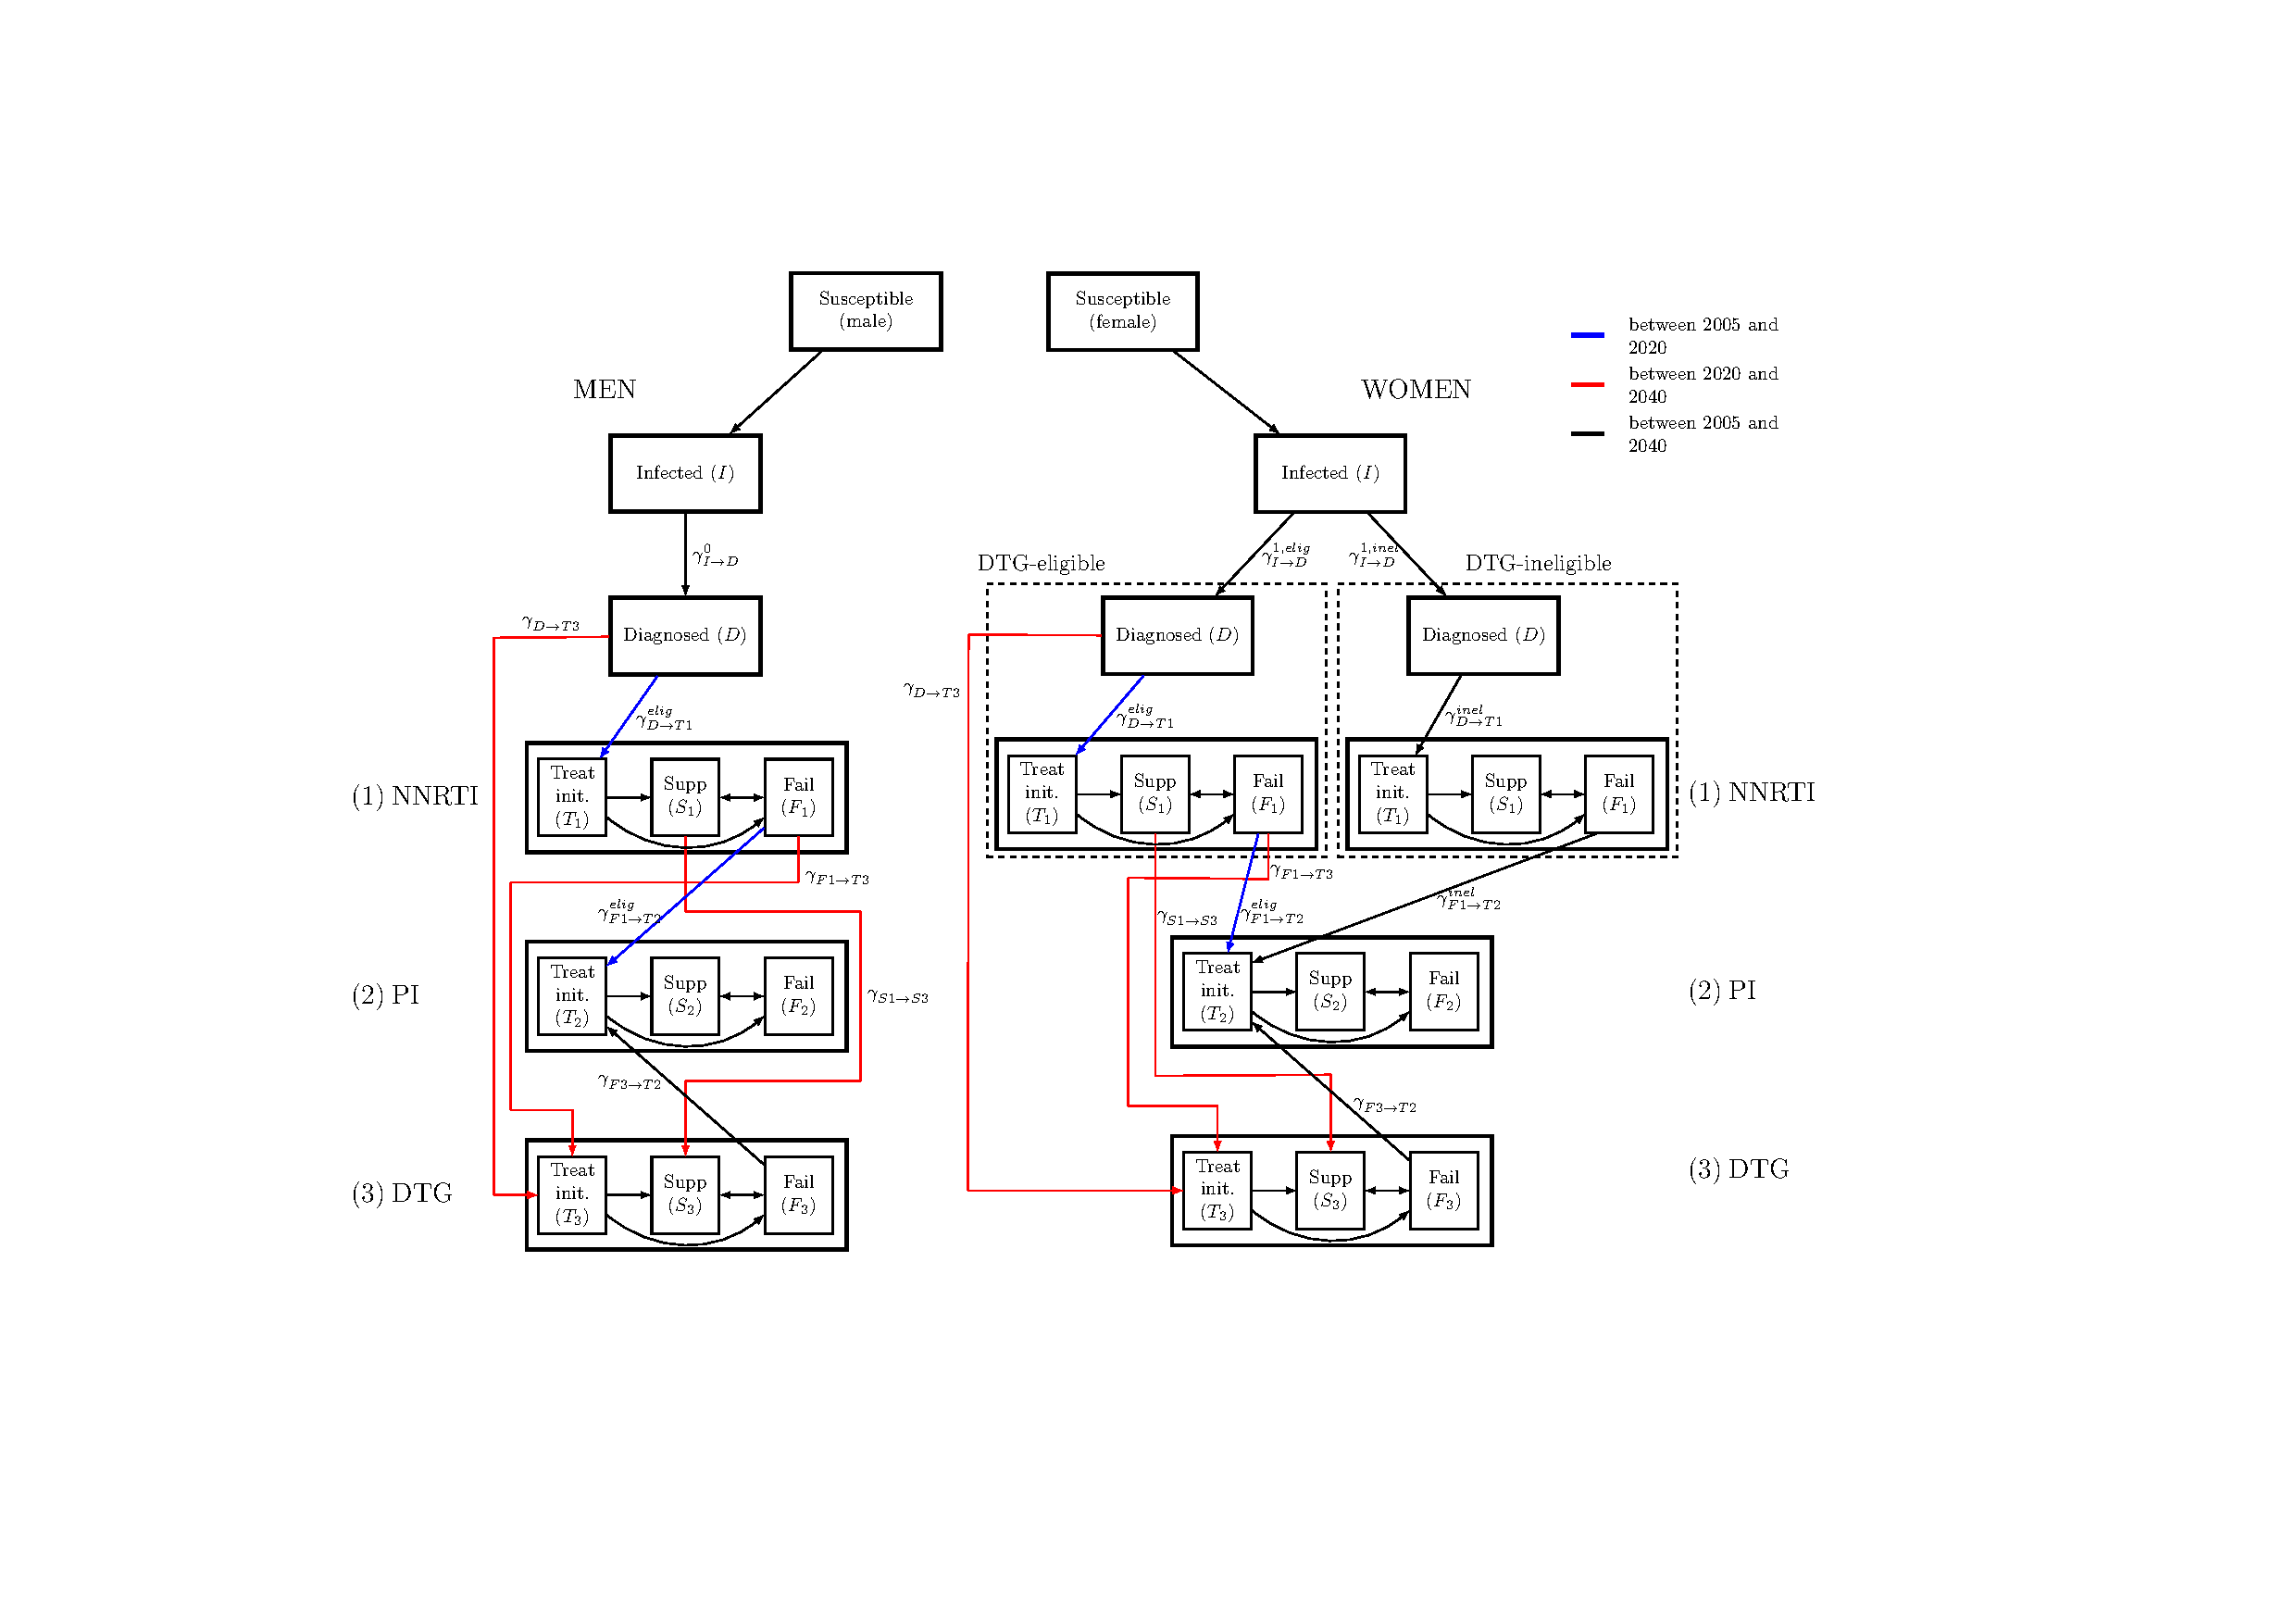
\includegraphics[width=14cm]{../figures/Fig1.pdf}
   \DIFaddendFL \vspace{0.5cm}
   \caption{{\bf The adapted MARISA model.}
The model differentiates DTG-eligible from DTG-ineligible women. The model structure related to the cascade of care is shown.}\label{fig1}
\end{figure}

We simulated the adapted model from 2005 to 2040 assuming the rollout of DTG-based ART started in \DIFdelbegin \DIFdel{2019 }\DIFdelend \DIFaddbegin \DIFadd{2020 }\DIFaddend under different scenarios (see below). We further assumed that all men and a proportion $p_1$ of women are eligible for DTG, this proportion varied between scenarios. Before \DIFdelbegin \DIFdel{2019}\DIFdelend \DIFaddbegin \DIFadd{2020}\DIFaddend , an NNRTI is used in first-line ART and PIs in second-line regimens. As first line regimen,  DTG is prescribed from \DIFdelbegin \DIFdel{2019 }\DIFdelend \DIFaddbegin \DIFadd{2020 }\DIFaddend on either to ART initiators (i.e. eligible, ART-naive people living with HIV) or for switching to DTG-based first-line ART (i.e. people on NNRTI and eligible for DTG). We assumed that patients failing DTG are switched to a PI-based regimen. For DTG-ineligible women, the cascade of care remains unchanged after \DIFdelbegin \DIFdel{2019 }\DIFdelend \DIFaddbegin \DIFadd{2020 }\DIFaddend (Fig \ref{fig1}).

\subsection*{Calibration and extension of the MARISA model}
We previously calibrated the MARISA model by combining different sources of data. Rates either related to treatment response (NNRTI- or PI-based regimen) or disease progression (characterized by CD4 counts) were estimated using clinical data from data from five cohorts in South Africa (Aurum Institute, Hlabisa, Khayelitsha, Kheth’Impilo and Tygerberg) that participate in the IeDEA collaboration  \cite{Egger2012}. These cohorts provided longitudinal information for 54,016 HIV-infected adults. Other parameters were either estimated from the literature (e.g. resistance-related parameters) or fitted to estimates from the Thembisa model (e.g. diagnosis rates and treatment initiation rates). Thembisa is a demographic projection model on which the official UNAIDS estimates for South Africa are based \cite{Johnson2017b}. More details about the calibration procedure can be found in \cite{Hauser2019} and in the supplementary materials (S1 Text, Section \DIFdelbegin \DIFdel{1.2}\DIFdelend \DIFaddbegin \DIFadd{1.1}\DIFaddend ).

We added and modified parameters in order to model the introduction of DTG. We assumed that the DTG initiation rate $\gamma_{D\rightarrow T3}^{}(t)$ is the same as the NNRTI initiation rate $\gamma_{D\rightarrow T1}^{}(t)$ from \DIFdelbegin \DIFdel{2019. }\DIFdelend \DIFaddbegin \DIFadd{2020. }\DIFaddend Both NNRTI and DTG initiation rates increase until 2022, as a consequence of the Treat-All policy that was implemented in 2017. From 2022 onwards, they are assumed to remain constant (S1 Text, Section \DIFdelbegin \DIFdel{2.1}\DIFdelend \DIFaddbegin \DIFadd{2.2}\DIFaddend ). Finally, we fixed switching rates from NNRTI- to DTG-based regimens for both eligible suppressed (see “Scenarios”) and all failing individuals ($\gamma_{S_1\rightarrow S_3}^{}(t)$ and $\gamma_{F_1\rightarrow T_3}^{}(t)$ respectively) to $1\text{ year}^{-1}$. \DIFdelbegin \DIFdel{Finally, we }\DIFdelend \DIFaddbegin \DIFadd{We }\DIFaddend assumed that suppressed individuals would stay suppressed when switching, while failing individuals would start DTG in the \textit{Treat init.} compartment (see Fig \ref{fig1}). The main parameters are summarized in Table \ref{table1}.

\newcolumntype{b}{X}
\newcolumntype{s}{>{\hsize=.6\hsize}X}
\newcolumntype{t}{>{\hsize=.5\hsize}X}
\newcolumntype{x}{>{\hsize=.041\hsize}X}
\newcommand{\heading}[1]{\multicolumn{1}{c}{#1}}
\newcommand\Tstrut{\rule{0pt}{2.8ex}}         % = `top' strut
\newcommand\Bstrut{\rule[-1ex]{0pt}{0pt}}

\begin{table}
\caption{\textbf{Main parameters used in the extended MARISA model.}}
\fontsize{7}{9}\selectfont
\centering
\renewcommand{\arraystretch}{1.5}
\begin{tabularx}{\textwidth}{xtsb}
\hline
&\textbf{Rate} & \textbf{Description} & \textbf{Source/Definition}\Tstrut\Bstrut\\
\hline
\multicolumn{4}{l}{\textit{\textbf{Rates estimated in the previous MARISA model \cite{Hauser2019}} }}\Tstrut\Bstrut\\[0.0cm]
 \rowcolor[gray]{0.94} \cellcolor{white}& $\gamma_{I\rightarrow D}^{k,elig/inel}$, $\gamma_{D\rightarrow T_1}^{k,elig}$ & Diagnosis rate, treatment initiation rate to NNRTI & Calibrated by fitting MARISA to Thembisa model (see \cite{Hauser2019}) from 2005 to 2016 (see S1 Text Section \DIFdelbeginFL \DIFdelFL{2.1 and Table 3}\DIFdelendFL \DIFaddbeginFL \DIFaddFL{2.2}\DIFaddendFL ) \\
& $\gamma_{T_1\rightarrow S_1}$,$\gamma_{T_1\rightarrow F_{1}}$, $\gamma_{F_1\rightarrow S_1}$,$\gamma_{S_1\rightarrow F_1}$ & NNRTI suppression and failure rates &Estimated with individual epidemiological data from IeDEA-SA \cite{Egger2012} (see S1 Text Table \DIFdelbeginFL \DIFdelFL{1}\DIFdelendFL \DIFaddbeginFL \DIFaddFL{2}\DIFaddendFL )\\
\rowcolor[gray]{0.94} \cellcolor{white} & $\gamma_{T_2\rightarrow S_2}$,$\gamma_{T_2\rightarrow F_{2}}$, $\gamma_{F_2\rightarrow S_2}$,$\gamma_{S_2\rightarrow F_2}$ & PI suppression and failure rates & Estimated with data from IeDEA-SA \cite{Egger2012} (see S1 Text Table \DIFdelbeginFL \DIFdelFL{1}\DIFdelendFL \DIFaddbeginFL \DIFaddFL{2}\DIFaddendFL )\\
 & $\gamma_{F_1\rightarrow T_2}^{k,elig/inel}$ & Rate of switching from NNRTI to PI (before \DIFdelbeginFL \DIFdelFL{2019}\DIFdelendFL \DIFaddbeginFL \DIFaddFL{2020}\DIFaddendFL ) & Estimated with data from IeDEA-SA and then adjusted (see S1 Text Section \DIFdelbeginFL \DIFdelFL{2.1}\DIFdelendFL \DIFaddbeginFL \DIFaddFL{2.2}\DIFaddendFL )\\
\multicolumn{4}{l}{\textbf{\textit{Added rates}}}\Tstrut\Bstrut\\
\rowcolor[gray]{0.94} \cellcolor{white} & $\gamma_{T_3\rightarrow S_3}$,$\gamma_{T_3\rightarrow F_3}$, $\gamma_{F_3\rightarrow S_3}$,$\gamma_{S_3\rightarrow F_3}$ & DTG suppression and failure rates & \DIFdelbeginFL \DIFdelFL{Assumption: same rate as for NNRTI (relaxed in }\DIFdelendFL \DIFaddbeginFL \DIFaddFL{Calibrated with data from NAMSAL study \mbox{%DIFAUXCMD
\cite{Group2019} }\hspace{0pt}%DIFAUXCMD
(see }\DIFaddendFL S1 Text Section \DIFdelbeginFL \DIFdelFL{5.1}\DIFdelendFL \DIFaddbeginFL \DIFaddFL{2.5}\DIFaddendFL )\\
& $\gamma_{D\rightarrow T3}^{}(t)$\hspace{0cm} (\DIFdelbeginFL \DIFdelFL{$t \geq 2019$}\DIFdelendFL \DIFaddbeginFL \DIFaddFL{$t \geq 2020$}\DIFaddendFL ) & DTG initiation rate (from \DIFdelbeginFL \DIFdelFL{2019}\DIFdelendFL \DIFaddbeginFL \DIFaddFL{2020}\DIFaddendFL ) & Same DTG initiation rate as for NNRTI (for DTG-inel. people) $\gamma_{D\rightarrow T3}^{}:=\gamma_{D\rightarrow T1}^{inel}$\Bstrut\\
\rowcolor[gray]{0.94} \cellcolor{white}& $\gamma_{I\rightarrow D}^{k,elig}(t)$,$\gamma_{I\rightarrow D}^{k,inel}(t)$,\hspace{2cm} \DIFdelbeginFL \DIFdelFL{$(t \geq 2019)$ }\DIFdelendFL \DIFaddbeginFL \DIFaddFL{$(t \geq 2020)$ }\DIFaddendFL & Diagnosis rate from \DIFdelbeginFL \DIFdelFL{2019 }\DIFdelendFL \DIFaddbeginFL \DIFaddFL{2020 }\DIFaddendFL (distribution across DTG-eligibility classes)& \DIFdelbeginFL \DIFdelFL{$\gamma_{I\rightarrow D}^{1,elig}(t)=p_1\cdot \gamma_{I\rightarrow D}^{1}(2019)$ and $\gamma_{I\rightarrow D}^{1,inel}(t)=(1-p_1)\cdot \gamma_{I\rightarrow D}^{1}(2019)$, for $t \geq 2019$ }\DIFdelendFL \DIFaddbeginFL \DIFaddFL{$\gamma_{I\rightarrow D}^{1,elig}(t)=p_1\cdot \gamma_{I\rightarrow D}^{1}(2020)$ and $\gamma_{I\rightarrow D}^{1,inel}(t)=(1-p_1)\cdot \gamma_{I\rightarrow D}^{1}(2020)$, for $t \geq 2020$ }\DIFaddendFL (see S1 Text Section \DIFdelbeginFL \DIFdelFL{2.1}\DIFdelendFL \DIFaddbeginFL \DIFaddFL{2.2}\DIFaddendFL )\\
& $\gamma_{F_1\rightarrow T_2}^{elig/inel}(t)$, \hspace{2cm} \DIFdelbeginFL \DIFdelFL{$(t \geq 2019)$ }\DIFdelendFL \DIFaddbeginFL \DIFaddFL{$(t \geq 2020)$ }\DIFaddendFL & Rate of switching from NNRTI to PI (DTG-inel.) & $\gamma_{F_1\rightarrow T_2}^{inel}(t)=\gamma_{F_1\rightarrow T_2}^{}$, $\gamma_{F_1\rightarrow T_2}^{elig}(t)=0$, for \DIFdelbeginFL \DIFdelFL{$t \geq 2019$ }\DIFdelendFL \DIFaddbeginFL \DIFaddFL{$t \geq 2020$ }\DIFaddendFL (see S1 Text Section \DIFdelbeginFL \DIFdelFL{2.1}\DIFdelendFL \DIFaddbeginFL \DIFaddFL{2.2}\DIFaddendFL )\\
\rowcolor[gray]{0.94} \cellcolor{white}& $\gamma_{F_3\rightarrow T_2}^{}(t),$ \DIFdelbeginFL \DIFdelFL{$(t \geq 2019)$ }\DIFdelendFL \DIFaddbeginFL \DIFaddFL{$(t \geq 2020)$ }\DIFaddendFL & Rate of switching from DTG to PI & $\gamma_{F_3\rightarrow T_2}^{}(t):=\gamma_{F_1\rightarrow T_2}^{inel}(t),$ \DIFdelbeginFL \DIFdelFL{$t \geq 2019$}\DIFdelendFL \DIFaddbeginFL \DIFaddFL{$t \geq 2020$}\DIFaddendFL \\
& $\gamma_{S_1\rightarrow S_3}^{}(t)$, \DIFdelbeginFL \DIFdelFL{$(t \geq 2019)$ }\DIFdelendFL \DIFaddbeginFL \DIFaddFL{$(t \geq 2020)$ }\DIFaddendFL & Switching rate from NNRTI to DTG (maintenance therapy) & $\gamma_{S_1\rightarrow S_3}^{k}(t):=1 \text{year}^{-1}$, \DIFdelbeginFL \DIFdelFL{$t \geq 2019$}\DIFdelendFL \DIFaddbeginFL \DIFaddFL{$t \geq 2020$}\DIFaddendFL \\
\rowcolor[gray]{0.94} \cellcolor{white}& $\gamma_{F_1\rightarrow T_3}^{}(t)$, \DIFdelbeginFL \DIFdelFL{$(t \geq 2019)$ }\DIFdelendFL \DIFaddbeginFL \DIFaddFL{$(t \geq 2020)$ }\DIFaddendFL & Switching rate from NNRTI to DTG (switch therapy) & $\gamma_{F_1\rightarrow T_3}^{}(t)=1\text{year}^{-1}$, \DIFdelbeginFL \DIFdelFL{$t \geq 2019$}\DIFdelendFL \DIFaddbeginFL \DIFaddFL{$t \geq 2020$}\DIFaddendFL \\
\hline
\end{tabularx}
\label{table1}
\end{table}

\DIFaddbegin \DIFadd{In the adapted MARISA model, we also added a fifth NRTI-resistance dimension to model the impact of NRTI-resistance on DTG-efficacy. NRTI-resistance is defined as having resistance to both tenofovir (TDF) and lamivudine/emtricitabine (3TC/FTC), the two backbones that are usually combined with DTG (see S1 Text, Section 2.5) \mbox{%DIFAUXCMD
\cite{RepublicofSouthAfricaNationalDepartmentofHealth2020}}\hspace{0pt}%DIFAUXCMD
. We assume that NRTI-resistance is acquired when failing NNRTI-based regimen. In view of the low levels of NRTI PDR that are observed in Africa and its rapid reversion to wild-type, we assumed as an approximation that it cannot be transmitted. We investigated different impacts of NRTI-resistance on DTG-based regimen and different DTG-efficacies. For this aim, we re-calibrated the model so that it reflects different odds ratios (ORs) of DTG-failure between NRTI-susceptible and NRTI-resistant individuals (OR=1, OR=2, OR=3). In the main analysis, we assumed that DTG-efficacy was similar to the one observed in the NAMSAL study, corresponding to an OR of failure between NNRTI and DTG of 1.02, after adjusting for the different baseline characteristics of the two groups (see S1 Text, Section 2.5). Other DTG efficacy corresponding to an OR of 2 and 5 were investigated in a supplementary analysis (see S1 Text, Section 5.3). All code and manuscript are available from }\url{https://github.com/anthonyhauser/MARISA2}\DIFadd{.
}


\DIFaddend \subsection*{Scenarios}\label{scen_section}
The model investigated the impact of the introduction of DTG-based regimens on the level of NNRTI resistance in diagnosed individuals \DIFaddbegin \DIFadd{(i.e. NNRTI PDR) }\DIFaddend under two main scenarios, with four variations for each of the two scenarios. We also examined the scenario where DTG-based ART is not introduced. There were thus nine scenarios in total. The two main scenarios were:
\begin{enumerate}
\item DTG only used in first-line regimen of ART-initiators and, as second-line, in patients failing NNRTI-based ART,
\item DTG used as initial first-line regimen (for ART-initiators), with all patients on NNRTI-based regimens being switched to a DTG-based regimen.
\end{enumerate}

\DIFaddbegin \DIFadd{For the second scenario, we varied the impacts of NRTI-resistance on DTG-based regimen, by successively assumed an OR of DTG-failure  between NRTI-resistant and -susceptible individuals of 1 (i.e. no impact) and of 2. }\DIFaddend Each scenario also investigated four different DTG eligibility levels $p_1$ for women. The population eligible for DTG in each scenario was:
\begin{enumerate}[label=\alph*)]
\item only men (100\% men, 0\% women)
\item men and women beyond reproductive age (100\% of men, 17.5\% of women)
\item men and women beyond reproductive age or using contraception (100\% of men, 63\% of women)
\item all men and women (100\% of men, 100\% of women)
\end{enumerate}
The percentages of women eligible for DTG in b) and c) were determined by analyzing cohort data from IeDEA, which show that 17.5\% adult women on ART are 50 or older \cite{Egger2012}, and estimates on the use of contraception from the World Bank \cite{WorldBank2015}(see S1 Text, Section 3.1). \DIFaddbegin \DIFadd{Throughout the rest of the paper, scenarios a) and b) will be referred as "men and women of childbearing age" and "men and women at risk of pregnancy", respectively. }\DIFaddend Of note, to model scenario 1., we set $\gamma_{S_1\rightarrow S_3}^{}(t)=0$ and $\gamma_{F_1\rightarrow T_3}^{}(t)=\gamma_{F_1\rightarrow T_2}^{inel}(t)$ (as opposed to scenario 2., where $\gamma_{S_1\rightarrow S_3}^{}(t)=\gamma_{F_1\rightarrow T_3}^{}(t)=1\text{ year}^{-1}$). We thus assumed that in all scenarios DTG will be used in second-line regimens for people failing NNRTI-based first-line ART.

\subsection*{Additional analyses}
We predicted the impact of different levels of DTG introduction on the level of NNRTI failure. We considered the scenario where DTG was prescribed to ART initiators and those on NNRTI-based first-line ART were switched to a DTG-based regimen, with the four different levels of women accessing DTG-based ART (see "Scenarios"). However, we assumed that 99\% of women were eligible for DTG in scenario d) (instead of 100\%), in order to estimate NNRTI failure when only a very small fraction of women rely on it. For each of these scenarios, we predicted the percentage of individuals failing an NNRTI-based regimen in different calendar years (2025 and 2035) and after different durations on ART (1 or 2 years). For each of the scenarios, we ran the model from 2005 up to 2035 and retained the numbers of people starting NNRTI-based first-line ART (by CD4 groups, NNRTI-resistance and gender) in 2025 and 2035. We then ran the model for the compartments related to NNRTI-treatment, using the previously saved starting values. This way, we could predict the levels of NNRTI-failure in patients starting NNRTI in either 2025 or 2035 after 1 or 2 years of ART.

We assessed the impact of different switching rates from NNRTI- to DTG-based regimens, fixed to $1 \text{ year}^{-1}$ for both suppressed and failing individuals. We varied both rates $\gamma_{S_1\rightarrow S_3}^{}(t)$ and $\gamma_{F_1\rightarrow T_3}^{}(t)$ within a range corresponding to a time to switch of between 0.5 and 10 $\text{years}$  after start of ART. For each analysis, the percentage of women who are DTG-eligible varied from $0\%$ to $100\%$.

\subsection*{Sensitivity analyses}
The values of eight parameters were varied in the sensitivity analysis: three transmission-related parameters (percentage of men who have sex with men (MSM), probability of male-to-male infection per sexual contact, and HIV prevalence ratio between MSM and heterosexuals), four resistance-related parameters (resistance rates, reversion to wild-type rate and the effect of NNRTI-resistance on NNRTI efficacy) and one parameter related to treatment (efficacy of DTG-based treatment). Multivariate uncertainty within specified ranges was assessed using Latin hypercube sampling \cite{Seaholm1988}. Each model estimate is reported with a 95\% sensitivity range. Further details are available in S1 Text, Section 3.2. \DIFaddbegin \DIFadd{and Fig 3 and 4.
}\DIFaddend In addition, we also investigated the impact \DIFdelbegin \DIFdel{of }\DIFdelend \DIFaddbegin \DIFadd{on NNRTI PDR of 1) }\DIFaddend lower treatment-initiation rates than suggested by the Treat-All policy (as suggested by \cite{Boyer2016}), \DIFdelbegin \DIFdel{treatment interruption and }\DIFdelend \DIFaddbegin \DIFadd{2) treatment interruption, 3) }\DIFaddend higher efficacy of DTG \DIFdelbegin \DIFdel{on NNRTI PDR }\DIFdelend \DIFaddbegin \DIFadd{and different impacts of NRTI-resistance on DTG }\DIFaddend (S1 Text, Section 5).

\section*{Results}
\subsection*{Use of NNRTIs and levels of resistance}
The percentages of patients treated with NNRTI and PI for each of the \DIFdelbegin \DIFdel{nine }\DIFdelend \DIFaddbegin \DIFadd{thirteen }\DIFaddend scenarios are shown in Fig \ref{fig2}. The predicted evolution of levels of NNRTI \DIFdelbegin \DIFdel{resistance }\DIFdelend \DIFaddbegin \DIFadd{PDR }\DIFaddend up to 2040 across the \DIFdelbegin \DIFdel{nine }\DIFdelend \DIFaddbegin \DIFadd{thirteen }\DIFaddend scenarios is shown in Fig \ref{fig3}. The model predicts that while NNRTI \DIFdelbegin \DIFdel{resistance }\DIFdelend \DIFaddbegin \DIFadd{PDR }\DIFaddend would increase substantially under continued NNRTI-based ART, the introduction of DTG-based ART can halt this increase, if in addition to starting new patients on a DTG-based regimen the patients on NNRTI-based regimens are switched to DTG-based first-line ART. Specifically, under the scenario of continued NNRTI-based ART as standard first-line therapy, NNRTI \DIFdelbegin \DIFdel{resistance }\DIFdelend \DIFaddbegin \DIFadd{PDR }\DIFaddend would increase to \blue\numberda (95\% sensitivity range: \blue\numberdb) by 2030 and \blue\numberea (\blue\numbereb) by 2040 (Fig \ref{fig3}A). At the other end of the spectrum, initiating all new ART patients on DTG-based ART and rapidly switching all patients currently on NNRTI-based ART to DTG-based regimens, independently of their gender, would stabilize NNRTI \DIFdelbegin \DIFdel{resistance at a low }\DIFdelend \DIFaddbegin \DIFadd{PDR at a moderate }\DIFaddend level, with a prevalence of \blue\numberfa (\blue\numberfb) by 2030 and \blue\numberga (\blue\numbergb) by 2040 (Fig \ref{fig3}B). \DIFaddbegin \DIFadd{When assuming an impact of NRTI-resistance on DTG-failure (Fig \ref{fig3}C), we found slightly higher levels of NNRTI PDR: }\blue\numberfc \DIFadd{(}\blue\numberfd\DIFadd{) in 2030 and }\blue\numbergc \DIFadd{(}\blue\numbergd\DIFadd{) in 2040, but a similar impact of the different scenarios of DTG introduction. }\DIFaddend Using DTG only in first-line regimens of patients initiating ART is not sufficient to curb the increase of NNRTI \DIFdelbegin \DIFdel{resistance}\DIFdelend \DIFaddbegin \DIFadd{PDR}\DIFaddend , even when given to all men and women (Fig \ref{fig3}A).

\DIFdelbegin %DIFDELCMD < \begin{figure}[h]
%DIFDELCMD <    %%%
%DIF < \includegraphics[width=14cm]{figures/t1.pdf}
   \DIFdelendFL \DIFaddbeginFL \begin{figure}[h!]
   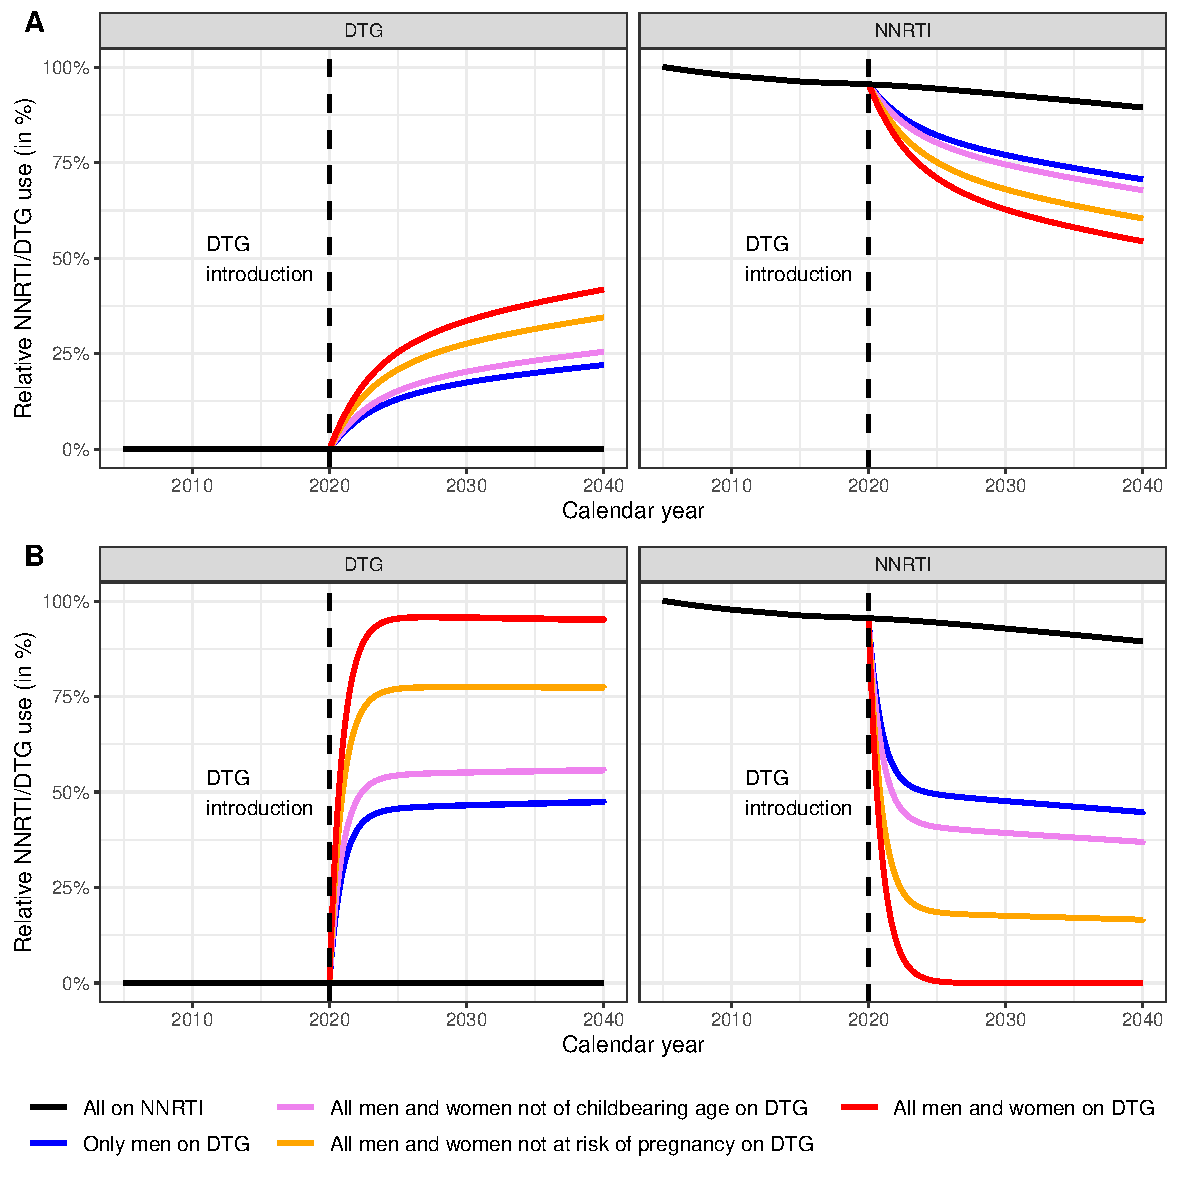
\includegraphics[width=14cm]{../figures/Fig2.pdf}
   \DIFaddendFL \vspace{0.5cm}
   \caption{{\bf Predicted use of NNRTI- and DTG-based regimens.}
Percentages of patients treated with NNRTI- and DTG-based regimens (left and right panels, respectively) are shown. Panels A represent the scenarios where DTG is used in patients initiating ART, while in panels B patients are also switched to DTG-based first line ART.}\label{fig2}
\end{figure}

\DIFdelbegin %DIFDELCMD < \begin{figure}[h]
%DIFDELCMD <    %%%
%DIF < \includegraphics[width=14cm]{figures/t2.pdf}
   \DIFdelendFL \DIFaddbeginFL \begin{figure}[h!]
   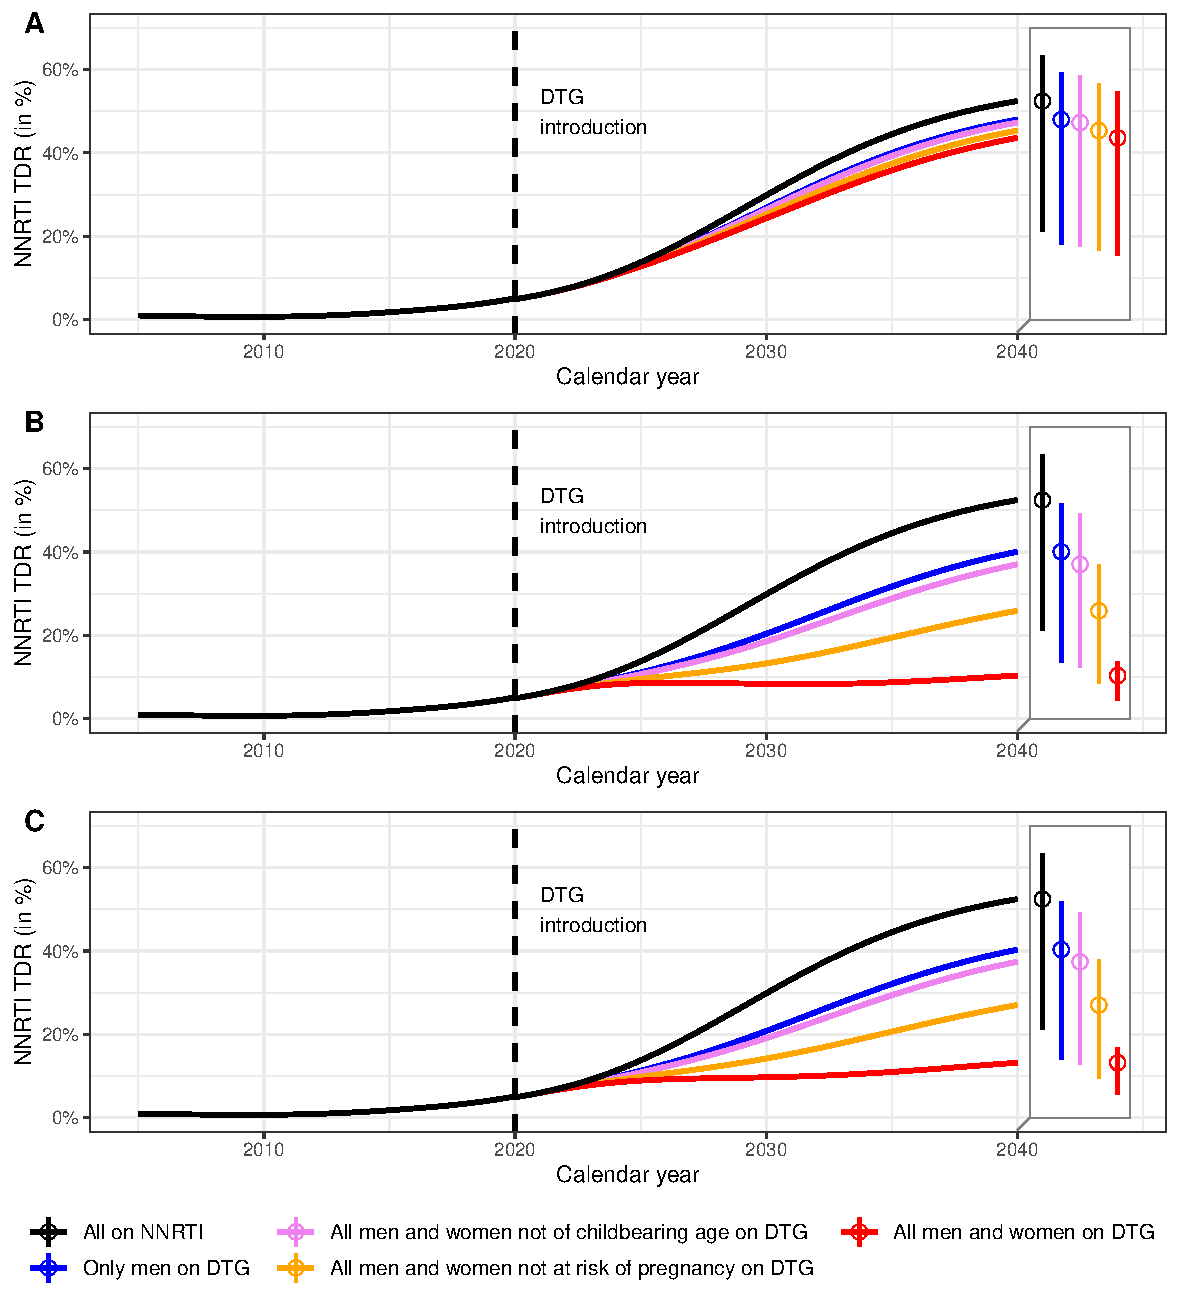
\includegraphics[width=14cm]{../figures/Fig3.pdf}
   \DIFaddendFL \vspace{0.5cm}
   \caption{{\bf Predicted levels of NNRTI pre-treatment drug resistance in South Africa (PDR) 2005-2040.}
Dolutegravir is introduced in \DIFdelbeginFL \DIFdelFL{2019 }\DIFdelendFL \DIFaddbeginFL \DIFaddFL{2020 }\DIFaddendFL under \DIFdelbeginFL \DIFdelFL{two }\DIFdelendFL \DIFaddbeginFL \DIFaddFL{three }\DIFaddendFL scenarios: DTG as first-line regimen for ART-initiators (panel A)\DIFdelbeginFL \DIFdelFL{or }\DIFdelendFL \DIFaddbeginFL \DIFaddFL{, }\DIFaddendFL DTG for all patients (panel B) \DIFaddbeginFL \DIFaddFL{or DTG for all patients}\DIFaddendFL , \DIFaddbeginFL \DIFaddFL{assuming an impact of NRTI-resistance on DTG-efficacy (panel C), }\DIFaddendFL and with different eligibility criteria for women \DIFaddbeginFL \DIFaddFL{(colors)}\DIFaddendFL . The baseline model shows the situation without the introduction of \DIFdelbeginFL \DIFdelFL{dolutegravir }\DIFdelendFL \DIFaddbeginFL \DIFaddFL{DTG }\DIFaddendFL (black line). The two boxes on the right of each panel represent the levels of NNRTI \DIFdelbeginFL \DIFdelFL{resistance }\DIFdelendFL \DIFaddbeginFL \DIFaddFL{PDR }\DIFaddendFL in 2040 and their 95\% sensitivity ranges.}\label{fig3}
\end{figure}

Restricting DTG-based ART to men to avoid the risk of DTG-associated \DIFdelbegin \DIFdel{neural tube defects }\DIFdelend \DIFaddbegin \DIFadd{NTD }\DIFaddend in newborns will not curb the increase in NNRTI \DIFdelbegin \DIFdel{resistance}\DIFdelend \DIFaddbegin \DIFadd{PDR}\DIFaddend : the prevalence of resistance is predicted to increase over the entire study period, reaching values of close to \DIFdelbegin \DIFdel{50}\DIFdelend \DIFaddbegin \DIFadd{4}\DIFaddend \% by 2040 (Fig \ref{fig3}B). The situation is similar under the scenario of initiating or switching men and women beyond childbearing age (17.5\% of women in the IeDEA cohorts). However, the model estimates that the increase in the prevalence of NNRTI \DIFdelbegin \DIFdel{resistance }\DIFdelend \DIFaddbegin \DIFadd{PDR }\DIFaddend is substantially slowed down if women beyond the age of reproduction or on contraception (63\% of women) also initiate a DTG-based regimen or switch to DTG. Under this scenario the prevalence of NNRTI \DIFdelbegin \DIFdel{resistance }\DIFdelend \DIFaddbegin \DIFadd{PDR }\DIFaddend is predicted to reach \blue\numberia (\blue\numberib) in 2040 (and \blue\numberha (\blue\numberhb) by 2030) if DTG is given to both ART-initiators and individuals already on NNRTI-based ART (Fig \ref{fig3}). \DIFaddbegin \DIFadd{Again, slightly higher NNRTI PDR levels are observed when including the impact of NRTI-resistance on DTG-efficacy: }\blue\numberic \DIFadd{(}\blue\numberid\DIFadd{) in 2040 and }\blue\numberhc \DIFadd{(}\blue\numberhd\DIFadd{) in 2030.
}\DIFaddend 

\subsection*{Impact of switching rates}
We calculated levels of NNRTI \DIFdelbegin \DIFdel{resistance }\DIFdelend \DIFaddbegin \DIFadd{PDR }\DIFaddend for 2035 for different average switching delays and percentages of women eligible for DTG-based ART\DIFaddbegin \DIFadd{, however without considering the effect of NRTI- resistance}\DIFaddend . We considered the effect of a modified switching rate both in suppressed individuals (Fig \ref{fig4}A) and in individuals on a failing regimen (Fig \ref{fig4}B). The predicted levels of NNRTI \DIFdelbegin \DIFdel{resistance }\DIFdelend \DIFaddbegin \DIFadd{PDR }\DIFaddend range from \blue\numberja to \blue\numberjb. The results indicate potential benefits of both strategies to reduce NNRTI resistance. However, as shown by the greater variation in the prevalence of NNRTI \DIFdelbegin \DIFdel{resistance }\DIFdelend \DIFaddbegin \DIFadd{PDR }\DIFaddend in the vertical than horizontal direction in Fig \ref{fig4}, allowing a higher proportion of women access to DTG-based ART has a greater impact than increasing switching rates.

\begin{figure}[h]
   %DIF < \includegraphics[width=14cm]{figures/t3_2.pdf}
   \DIFaddbeginFL 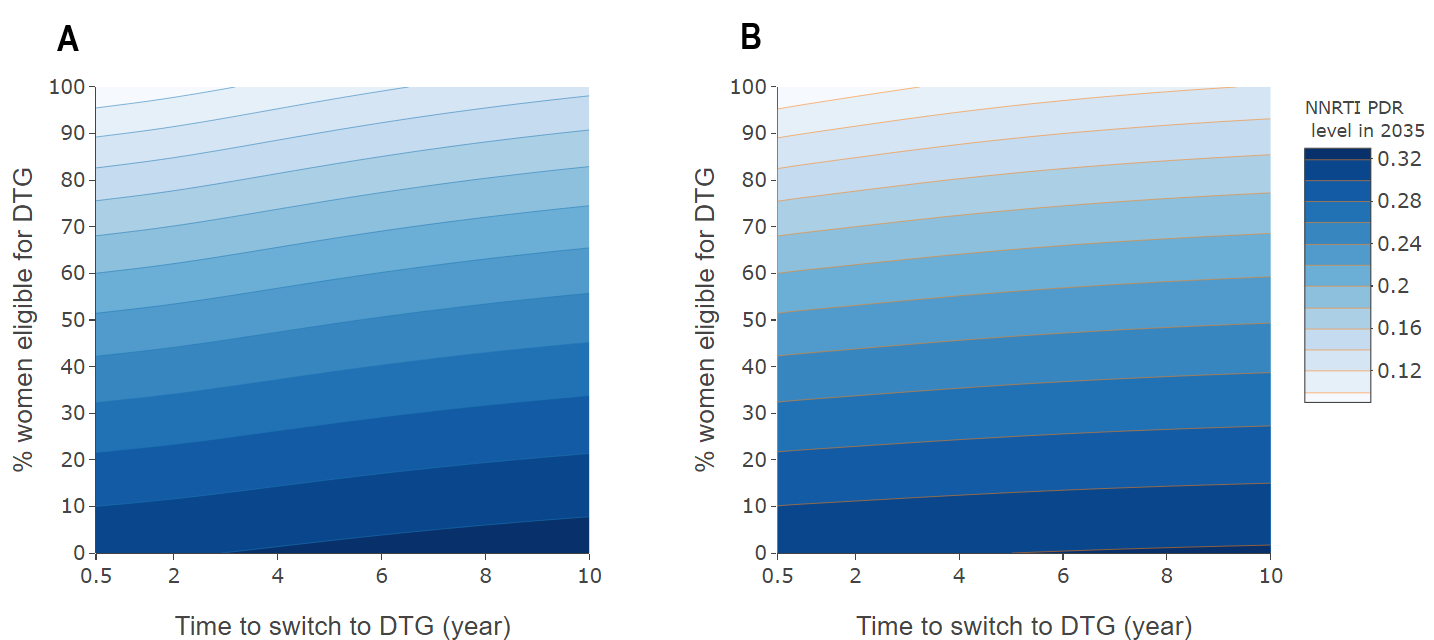
\includegraphics[width=14cm]{../figures/Fig4r.png}
   \DIFaddendFL \vspace{0.5cm}
   \caption{{\bf Level of NNRTI pre-treatment drug resistance in 2035, by rate of switching to DTG-based ART and percent women eligible for DTG-based ART.}
Panel A relates to patients on first-line ART with suppressed HIV-1 replication, and panel B to individuals failing NNRTI-based ART. The average time to switching (i.e. the inverse of the switching rate) varies from 0.5 to 10 years for individuals with viral suppression (panel A) or failure (panel B).}\label{fig4}
\end{figure}
\subsection*{Impact of DTG-eligibility on the rate of NNRTI failure}
As expected from their effect on NNRTI resistance, the different scenarios of the rollout of DTG-based ART also influence the
\DIFdelbegin \DIFdel{rate of virological failure in women }\DIFdelend \DIFaddbegin \DIFadd{virological failure under }\DIFaddend NNRTI-based ART\DIFdelbegin \DIFdel{among DTG-ineligible. We find that the proportion }\DIFdelend \DIFaddbegin \DIFadd{. Fig \ref{fig5} shows the predicted proportion of NNRTI-failure after 1 and 2 years among DTG-ineligible women according to different scenarios }\DIFaddend of \DIFdelbegin \DIFdel{NNRTI failure is increasing over calendar time of ART start for all scenarios , as a result of the increase of NNRTI resistance among NNRTI-initiators (see Fig \ref{fig5}, 2025 vs 2035)}\DIFdelend \DIFaddbegin \DIFadd{DTG-introduction}\DIFaddend .
In the absence of DTG introduction, we observe a high level of failure in women starting NNRTI in 2035, reaching \blue\numberk after 2 years of ART. \DIFdelbegin \DIFdel{Providing all men with DTG}\DIFdelend \DIFaddbegin \DIFadd{If all men are started on or switched to DTG, it }\DIFaddend would help diminish the level of failure by 2 years to \blue\numberl in \DIFdelbegin \DIFdel{2035. }\DIFdelend \DIFaddbegin \DIFadd{2035, and to }\blue\numberlb \DIFadd{when including the impact of NRTI-resistance. }\DIFaddend This percentage decreases to \blue\numberm, when including all women not at risk of pregnancy \DIFaddbegin \DIFadd{(}\blue\numbermb \DIFadd{when including NRTI-resistance)}\DIFaddend , and to \blue\numbern \DIFaddbegin \DIFadd{(}\blue\numbernb \DIFadd{when including NRTI-resistance) }\DIFaddend if all men and 99\% of women are included. Therefore, we find that the increase of virological failure in DTG-ineligible women who still rely on NNRTI can be stopped by the introduction of DTG.

\begin{figure}[h]
%DIF < \includegraphics[width=14cm]{figures/t4.pdf}
\DIFaddbeginFL 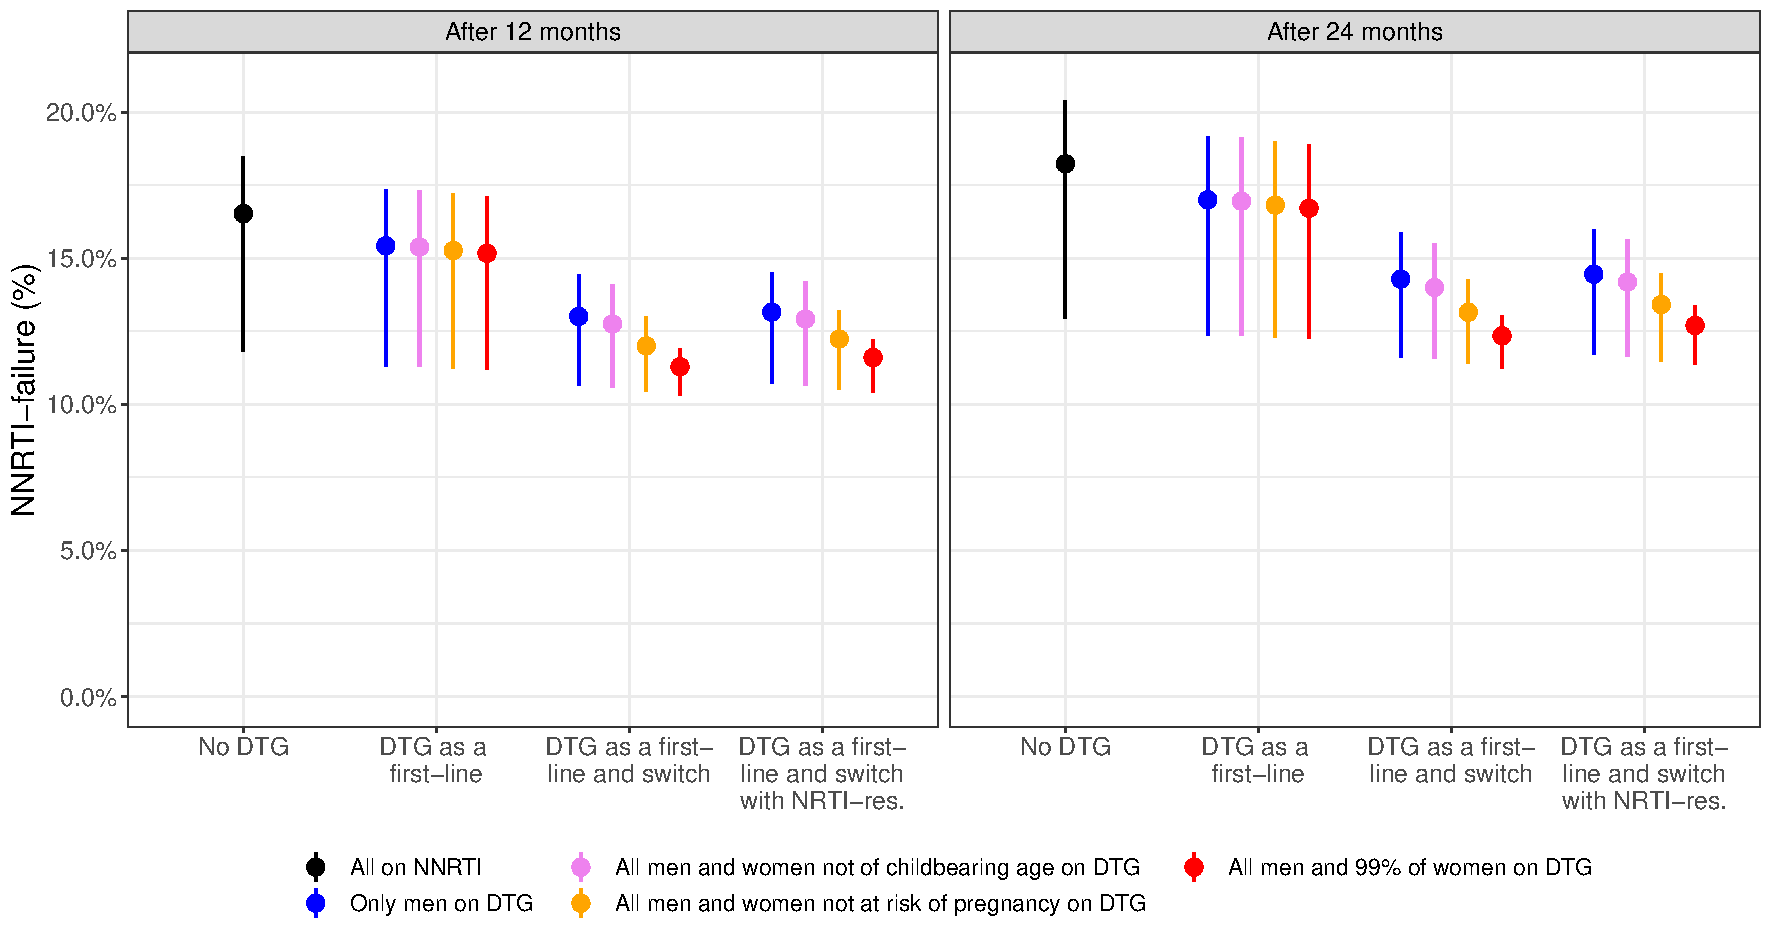
\includegraphics[width=14cm]{../figures/Fig5.pdf}
\DIFaddendFL \vspace{0.5cm}
\caption{{\bf Predicted percentage of women failing NNRTI-based ART after one and two years of ART in 2025 and 2035, depending on the scenario of the rollout of DTG-based ART.} Note that the scenario in which DTG is given to all men and 99\% of women (in red) replaces the scenario in which DTG was given to all men and women (see "Additional analyses"). Failure is given after 1 and 2 years of ART.}\label{fig5}
\end{figure}

\section*{Discussion}
We adapted the epidemiological MARISA model to examine the impact of the scale-up of DTG-based ART on NNRTI pre-treatment drug resistance in South Africa. Overall, our findings suggest that if a large fraction of women is excluded from receiving DTG-based ART, they will not only receive a potentially inferior NNRTI-based regimen but will also face increasing rates of resistance to this regimen due to the population level effects of continued NNRTI use. In contrast, the spread of NNRTI-resistance can be slowed down if DTG-based ART is made accessible both to women at low risk of pregnancy and to people currently on a NNRTI-based first-line regimen, thereby indirectly protecting those still requiring a NNRTI-based treatment. Model simulations emphasize the importance \DIFaddbegin \DIFadd{of }\DIFaddend starting on or switching a maximum number of women to DTG-based ART: increasing use of DTG-based regimens was the strategy with the greatest potential to curb the spread of NNRTI resistance. The latter strategy will also lower the risk of virologic failure in women who have to rely on NNRTI-based ART in the future. \DIFaddbegin \DIFadd{Finally, it is interesting to observe that, even when using DTG for everybody, NNRTI PDR still remains approximatively stable at a moderate level, due to the very slow reversion of NNRTI-resistance that allows subsequent transmission of NNRTI-resistance (in line with \mbox{%DIFAUXCMD
\cite{Yang2015}}\hspace{0pt}%DIFAUXCMD
).
}\DIFaddend 

While some countries, such as South Africa, first considered to limit access to DTG to men, menopausal women, and women using long-term family planning as a potential policy, the new WHO guidelines state that women should not in principle be excluded from DTG-based ART, even women who are at risk of pregnancy or desire to get pregnant. WHO recommends a woman-centered approach where women should be provided with information about benefits and risks to make an informed choice \cite{Milanga2018,WHO2019}. It is unclear what proportion of women will effectively receive DTG-based ART, as it depends on individual women’s decisions. In this context, model simulations are essential in order to assess the impact of the different options proposed and different levels of DTG uptake. A strength of our model is that it deals with the two most significant sources of uncertainty associated with the introduction of DTG, namely DTG uptake in women and the delay in switching people currently on NNRTI regimens. Despite the uncertainty concerning the uptake of DTG in women, it is likely that a proportion of women will continue to rely on NNRTI-based ART. Therefore, even with the rollout of DTG, NNRTI resistance will continue to be relevant for these women. Compared with other modelling work that assessed risks and benefits of DTG introduction (e.g. \cite{Dugdale2019}), our model focused on its indirect, population-level impact on NNRTI resistance. Rather than assigning a level of NNRTI resistance that is fixed over time, HIV care and disease stages (as in \cite{Dugdale2019}), our model considered the dynamic development of NNRTI resistance under relevant scenarios.

Our model also has several limitations. First, real-world data on the efficacy of DTG, especially in resource-limited settings are scarce. Therefore, we conservatively assumed that DTG has a similar efficacy as \DIFdelbegin \DIFdel{NNRTI. The effect of higher DTG efficacy, as suggested by several studies \mbox{%DIFAUXCMD
\cite{Group2019,Venter2019}}\hspace{0pt}%DIFAUXCMD
, is }\DIFdelend \DIFaddbegin \DIFadd{observed in the NAMSAL study \mbox{%DIFAUXCMD
\cite{Group2019}}\hspace{0pt}%DIFAUXCMD
. Higher DTG efficacies as well as different impacts of NRTI-resistance on DTG-failure are }\DIFaddend investigated in supplementary analyses (see S1 Text, Section 5.3). Second, predictions of levels of NNRTI resistance over the next twenty years are naturally uncertain, as reflected by the wide sensitivity ranges in Fig \ref{fig3}. However, despite the uncertainty, it is clear that the different strategies of rolling out DTG-based ART influenced the levels of NNRTI resistance. Finally, the MARISA model includes some simplifying assumptions, e.g. we did not model prevention of mother to child transmission (PMTCT), or treatment interruption. However, relaxing some of these assumptions did not drastically change our conclusion (see S1 Text, Section 5).

Another limitation of this study is the fact that the MARISA model does not take into account \DIFdelbegin \DIFdel{resistances to neither NRTI nor DTG }\DIFdelend \DIFaddbegin \DIFadd{resistance to DTG and uses a simplified representation of NRTI-resistance}\DIFaddend . In the context of the introduction of DTG-based ART, modelling of NRTI resistance is particularly relevant as individuals starting on DTG as a functional monotherapy due to resistance to both NRTI backbones - tenofovir and lamivudine - experience higher risk of treatment failure \cite{Wandeler2019}. As they are considerably less frequently transmitted \cite{WHO2017} and revert back quickly \cite{rev,Kuhnert2018}, NRTI resistances might primarily be an issue for ART-experienced individuals and more specifically, in patients failing NNRTI-based regimens, who often exhibit high levels of NRTI resistance \cite{Steegen2017}. These patients who are on non-suppressive NNRTI-based regimens are expected to switch to DTG, either after identification of treatment failure, following the new WHO guidelines, or blindly \cite{Inzaule2019}. In the context of modelling the DTG rollout, this consideration has two important implications. First, patients currently failing NNRTI-based regimens are expected to have higher DTG failure rates, mainly due to previously acquired NRTI resistance. Second, due to ongoing viral replication and due to pre-existing NRTI resistance, they are at higher risk of accumulating resistance, which may also lead to the emergence of DTG resistance. So far, data on emergence of DTG resistance is primarily available from patients in whom treatment failure was detected relatively early, which may not be the case in African settings \cite{Venter2019}. Therefore, to understand risk inherent in the emergence of DTG resistance, adapting the MARISA model by extending its resistance dimension to \DIFdelbegin \DIFdel{both NRTI and DTG resistances }\DIFdelend \DIFaddbegin \DIFadd{DTG resistance }\DIFaddend will be necessary.

\section*{Conclusion}
In conclusion, our study indicates that giving access to DTG-based ART to all women not at risk of pregnancy could limit the increase of NNRTI \DIFdelbegin \DIFdel{resistance}\DIFdelend \DIFaddbegin \DIFadd{PDR}\DIFaddend , but even if all women receive DTG-based ART the level of NNRTI \DIFdelbegin \DIFdel{resistance }\DIFdelend \DIFaddbegin \DIFadd{PDR }\DIFaddend will remain above 10\% in South Africa. Our model highlights the importance of a rapid switch of patients currently on NNRTI-based to DTG-based ART in order to limit the increase in NNRTI \DIFdelbegin \DIFdel{resistance}\DIFdelend \DIFaddbegin \DIFadd{PDR}\DIFaddend . Women who remain on NNRTI-based ART will indirectly benefit from a high level of DTG uptake due to a reduced risk of virologic failure. 

\DIFaddbegin \section*{\DIFadd{Acknowledgements}}
\DIFadd{Computations were conducted on UBELIX (}\url{http://www.id.unibe.ch/hpc}\DIFadd{), the high performance computing cluster at the University of Bern, Switzerland.
}

\nolinenumbers

\bibliography{C:/Users/ahauser/Documents/Step2/Step2_revised/dtg_latex_roger/dtg_bib}


\DIFaddend \section*{Supporting information}

\paragraph*{S1 Text}
\label{s1_file}
{\bf Supplementary Material.} Section 1: description of the \DIFdelbegin \DIFdel{previous  }\DIFdelend \DIFaddbegin \DIFadd{adapted }\DIFaddend MARISA model. Section 2: description of \DIFdelbegin \DIFdel{the adapted MARISA model }\DIFdelend \DIFaddbegin \DIFadd{model parameters}\DIFaddend . Section 3: \DIFdelbegin \DIFdel{detailed description of the additional and sensitivity analyses}\DIFdelend \DIFaddbegin \DIFadd{Model simulation}\DIFaddend , Section 4: Model equations. Section 5: Additional \DIFaddbegin \DIFadd{results and }\DIFaddend sensitivity analyses.
 \DIFdelbegin %DIFDELCMD < 

%DIFDELCMD < \nolinenumbers
%DIFDELCMD < 

%DIFDELCMD < \newpage
%DIFDELCMD < %%%
%DIF < \bibliography{dtg_bib}
%DIFDELCMD < \bibliography{C:/Users/ahauser/Documents/Step2/dtg_latex_roger/dtg_bib}
%DIFDELCMD <  %%%
\DIFdelend\end{document}

